\documentclass[11pt, twocolumn]{article}
\usepackage{../../latex/preamble}

\newcommand{\abs}[1]{|#1|}
\begin{document}
  % make title page
\begin{titlepage}
  \newcommand{\HRule}{\rule{\linewidth}{0.5mm}}
  \center
  \textsc{\LARGE Universitetet i Oslo}\\[1.5cm] % Name of your university/college
  \textsc{\Large }\\[0.5cm] % Major heading such as course name
  \textsc{\large FYS3150}\\[0.5cm] % Minor heading such as course title
  \HRule \\[0.4cm]
  { \huge \bfseries En titt på Isingmodellen og dens applikasjoner
  på termodynamiske størrelser}\\[0.4cm]
  \HRule \\[1.5cm]
  \Large \emph{Skrevet av:}\\
  Lyder \textsc{Rumohr Blingsmo} (k.nr. 2) og Bendik \textsc{Samseth} (k.nr. 27)\\[3cm]
  {\large \today}\\[3cm]
  \vfill
\end{titlepage}
\twocolumn[
\begin{@twocolumnfalse}
\tableofcontents
\vspace{\baselineskip}
\begin{abstract}
I denne rapporten har vi sett på Ising-modellen i to dimensjoner. Spesielt ser vi
på de termodynamiske egenskapene til et system under denne modellen, og hvordan disse
oppfører seg rundt den kritiske temperaturen. Vi bruker Metropolis-algoritmen med 
'periodic boundary conditions' for å gjøre simuleringene. Vi har også
sett på effekten av termalisering på forventningsverdiene som regnes
ut. Til slutt estimerer vi den kritiske temperaturen i den
termodynamiske grensen. Vi ender opp med et akseptabelt estimat, men
ser at vi gjerne skulle hatt tid til å gjøre mer nøyaktige
(tidkrevende) beregninger. Alt materiale som har blitt referert er tilgjengelig 
på Github~\cite{github-repo}. 
\end{abstract}
\vspace{\baselineskip}
\end{@twocolumnfalse}
]


\section{Innledning}
\label{sec:innledning}
Ising-modellen har mange praktiske applikasjoner. Den ble utviklet som en
beskrivelse av magnetisme i krystaller, men kan også anvendes på så vidt
forskjellige ting som frysning og fordampning av væsker, folding av 
protein-molekyler og oppførselen av 'glassy substances'~\cite{nature-ising}.

Modellen består av et system av $L \times L$ partikler ordnet i et rutenett. 
Hver partikkel kan være i én av to tilstander, enten spinn opp, $\uparrow$,
eller spinn ned, $\downarrow$. Energien er gitt ved 

\begin{equation}
  E=-J\sum_{<kl>}^{N}s_ks_l\label{eq:energi}
\end{equation}
der  $s_k=\pm 1$, $N = L^2$ er antall partikler.
$J$ er en konstant som beskriver styrken på interaksjonen mellom
nabopartikler. Symbolet $<kl>$ betyr at vi summerer over bare de
nærmeste naboene. Vi antar ferromagnetisme, dvs.  $J> 0$, og bruker også
periodiske randbetingelser. Det betyr at partiklene langs randa 'ser' 
partiklene langs motsatte rand. For eksempel 'ser' en partikkel i posisjon
(L,L) i rutenettet, både partikkelen i posisjon (1,L) og (L,1), og interakterer
med disse som om de skulle vært naboer. Dette tilsvarer at vi har
gitterstruktur, der systemet vi ser på gjentas videre i alle
retninger. Når vi har energien kan vi definere noen termodynamiske størrelser:

\begin{align}
Z &= \sum_i e^{-\beta E(i)} = \sum_E \Omega(E) e^{-\beta E}\label{eq:partisjons-funk} \\
C_V &= \frac{ 1 }{ k_B T^2} \left( \mean{E^2}-\mean{E}^2 \right)\label{eq:spesifikk-varmekapasitet} \\
\mathcal{M} &= \sum_i s_i\label{eq:magnetisering} \\
\chi &= \frac{ 1 }{ k_BT } \left( \mean{\mathcal{M}^2} - \mean{\mathcal{M}}^2 \right)\label{eq:susceptibilitet}.
\end{align}

Her er $\beta = 1/k_BT$, $Z$ partisjonsfunksjonen, $C_v$ er den spesifikke varmekapasiteten,
$\mathcal{M}$ er magnetiseringen og $\chi$ er susceptibiliteten. $E$, $T$ og $k_B$ er henholdsvis 
energien, temperaturen og boltzmannkonstanten. Disse størrelsene skal vi regne ut for flere forskjellige
størrelser på rutenettet og for mange forskjellige temperaturer.


\section{Implementering og testing}

Vi har tatt utgangspunkt i eksempelprogrammet \texttt{MPIising.cpp}
som finnes på kursets Github-side~\cite{compphys-github}. Versjonen brukt
i denne rapporten er tilgjengelig på Github~\cite{github-repo} under samme navn. Kjernen av
programmet er Metropolisalgoritmen, som i vårt tilfelle går som følger: 

\begin{enumerate}
\item Initialiser en vilkårlig starttilstand med energi $E_0$, dvs. 
bestem retningen på alle spinn i systemet. 
\item Velg en tilfeldig spinn og snu den.\label{steg2}
\item Beregn endringen i energi, $\Delta E = E_1-E_0$, dette fører til.\label{steg3} 
\item Dersom $\Delta E \leq 0$ godtar vi spinnendringen i håp om at vi
  er nærmere den minste mulige verdien av $E$. Gå til punkt (\ref{steg7}).
\item Dersom $\Delta E > 0 $, beregn Boltzmann-sannsynligheten $w = e^{-\beta\Delta E}$. 
\item Sammenlikn $w$ med et tilfeldig tall $0\leq r\leq 1$ \label{steg6}
\begin{enumerate}
  \item Hvis $r\leq w$, godta spinnendringen
  \item ellers, behold den originale spinntilstanden.
\end{enumerate}
\item Oppdater relevante forventningsverdier og gjenta prosessen\label{steg7}
  $N^2$ ganger, der $N^2$ er antall spinn.\footnote{Egentlig bare $N^2-1$ ganger fordi vi nå har gjort en
  allerede.}
\item Gjenta så steg (\ref{steg2})-(\ref{steg7}) mange ganger, der hver gjennomgang teller som
  én Monte Carlo-syklus.
\end{enumerate}

I steg (\ref{steg3}) beregner vi energiendringen. Når vi kun endrer på
én spinn om gangen er det kun 5 mulige verdier for $\Delta E$ for en
gitt verdi av $T$~\cite[s. 436]{Lecture-notes}. Derfor velger vi å
regne ut disse på forhånd og heller slå opp riktig verdi ved
behov. Dette gjør vi for å spare oss for mange gjentatte kall på \texttt{exp()}. Vi regner alle de termodynamiske størrelsene
i ligning \eqref{eq:partisjons-funk} - \eqref{eq:susceptibilitet} enhetsløst. 
 Som inputparametre tar vi størrelsen på rutenettet, antall Monte Carlo-sykluser,
initiell temperatur, sluttemperatur, temperatursteg og en parameter som bestemmer om den initielle
spinkonfigurasjonen er tilfeldig eller ordnet med alle spinn pekende ned. Koden er parallellisert med Open MPI. \footnote{Vi har konsekvent kjørt med fire
prosesser. Hver prosess kjører en uavhengig Ising-modell, med en fjerdedel av det totale antall Monte Carlo-sykluser. }

\subsection{Test med $2 \times 2$-tilfellet}
For å få en intuisjon om hvordan et slikt system fungerer ser vi først på 
$2 \times 2$-tilfellet. Her kan vi finne en eksakt løsning, og det er en god test
av programmet vårt å sammenligne med denne. Vi ser for oss et rutenett av spinn
\begin{align*}
s_1 & s_2 \\
s_3 & s_4  
\end{align*}

Vi får da energien

\begin{align*}
E &= -J ( s_1s_2 + s_1s_3 + s_2s_1 + s_2s_4 \\
&  \hspace{1.1cm}+ s_3s_1 + s_3s_4 + s_4s_ + s_4s_3) \\ 
&= - J  ( 2s_1s_2 + 2s_1s_3 + 2s_2s_1 + 2s_2s_4 ) 
\end{align*}

Bruker vi spinn-konfigurasjonen
\begin{align*}
\uparrow & \uparrow \\
\uparrow & \uparrow
\end{align*}

Får vi energien 
\begin{align*}
E &= - J  ( 2s_1s_2 + 2s_1s_3 + 2s_2s_1 + 2s_2s_4 ) \\&= -J ( 8 \cdot 1 \cdot 1) = -8J  
\end{align*}
Gjør tilsvarende for alle mulige spinn-konfigurasjoner får vi tabell \ref{tab:spinn-energi-deg}:


\begin{table*}[ht]
\centering
\caption{Tabell over energiene og degenerasjonene til de ulike
  spinn-konfigurasjonene til et $2\times 2$-rutenett av spinn.}
\label{tab:spinn-energi-deg}
\vspace{0.5cm}
\begin{tabular}{cccc}
Antall spinn opp & Degenerasjon & Energi & Magnetisering \\
\hline
4 & 1 & -8J & 4 \\
3 & 4 & 0 & 2 \\
2 & 4 & 0 & 0 \\
2 & 2 & 8J & 0 \\
1 & 4 & 0 & -2 \\
0 & 1 & -8J & -4 \\
\hline
\end{tabular}
\end{table*}

Vi ser av tabell \ref{tab:spinn-energi-deg} at energien kan ha tre
mulige verdier, $E = -8J,0,8J$. Da er partisjonsfunksjonen gitt ved
likning (\ref{eq:partisjons-funk}) (bruker også degenerasjonsgradene
oppgitt i tabellen):
\begin{align}
  Z &= \sum_E \Omega(E)e^{-\beta E}\\ &= 2e^{-\beta \cdot 8J} + 2e^{\beta
  \cdot 8J} + 12\label{eq:partisjons-funk-2x2}
\end{align}
Med partisjonsfunksjonen i boks kan vi finne alle forventningsverdier.

\begin{align}
\begin{split}
  \mean{E} &= \frac{ 1 }{ Z }\sum_E \Omega(E) E e^{-E\beta}\\
           &= 8J \frac{ e^{-8J\beta}  - e^{8J\beta}}{ e^{-8J\beta}
             + e^{8J\beta} + 6}\label{eq:mean-E-2x2}
\end{split}
\end{align}
\begin{align}
\begin{split}
  \mean{E^2} &= \frac{ 1 }{ Z }\sum_E E^2\Omega(E)e^{-E\beta}\\
  &= 64J^2 \frac{ e^{8J\beta} + e^{-8J\beta} }{ e^{-8J\beta} +
    e^{8J\beta} + 6 }\label{eq:mean-E2-2x2}
\end{split}
\end{align}
\begin{align}
  C_V &= \frac{ 1}{k_BT^2} \left( \mean{E^2} - \mean{E}^2
        \right)\label{eq:mean-C-2x2}
\end{align}
\begin{align}
\begin{split}
  \mean{|\mathcal{M}|} &= \frac{ 1 }{ Z }\sum_i |\mathcal{M}_i| e^{-E_i\beta}\\
  &= \frac{ 4e^{8J\beta} + 8  }{ e^{-8J\beta} + e^{8J\beta} + 6 }.\label{eq:mean-abs-M-2x2}
\end{split}
\end{align}
\begin{align}
\mean{\mathcal{M}} &= 0\label{eq:mean-M-2x2}
\end{align}
\begin{align}
\begin{split}
  \mean{\mathcal{M}^2} &= \frac{ 1 }{ Z } \sum_i \mathcal{M}^2
  e^{-E_i\beta}\\
  &= 16 \frac{ e^{8J\beta} + 1 }{ e^{8J\beta} + e^{-8J\beta}+6 }\label{eq:mean-M2-2x2}
\end{split}
\end{align}
\begin{align}
\mean{\chi} &= \frac{ 1 }{ k_B T} \left(
              \mean{\mathcal{M}^2}-\mean{\mathcal{M}}^2
              \right)\label{eq:mean-chi-2x2}\\[0.5cm]
\mean{\chi}_\text{abs} &= \frac{ 1 }{ k_B T} \left( \mean{\mathcal{M}^2}-\mean{\mathcal{|M|}}^2 \right)\label{eq:mean-chi-2x2-abs}
\end{align}

Vi kan nå bruke disse formlene til å teste programmet. Vi velger å se
på $T=1$.\footnote{Gjennom hele rapporten har vi gjort alle
  størrelser dimensjonsløse med $J=k_B=1$.} Tabell \ref{tab:2x2-eksakt-num} viser både eksakte og
numeriske resultater. Etter litt testing kom vi frem til at ca. $10^6$
Monte Carlo-sykluser gir god overensstemmelse (dette gjelder for å få
bra verdier for \textit{alle} størrelser. F.eks. energien ser ut til å bli bra
raskere enn f.eks. $C_V$).


\begin{table*}
\centering
\caption{Tabell over eksakte og numeriske resultater for $2\times
  2$-tilfellet for $T=1$. Vi har brukt $10^6$ Monte Carlo-sykluser og
  en startkonfigurasjon med alle spinn pekende ned, $\downarrow$. Merk at
alle tall er normalisert for antall spinn.}
\label{tab:2x2-eksakt-num}
\vspace{0.1cm}
\begin{tabular}{l|ccccc}
$T=1$ & $\mean{E}$ & $\mean{ \abs{\mathcal{M} } }$ & $C_V$ & $\chi$ & $\chi_\text{abs}$ \\
\hline
Eksakt & -1.9959821 & 0.99866073 & 0.032082332 & 3.9933038 & 0.0040107395 \\
Numerisk & -1.9960480 & 0.99869100 & 0.031585527 & 3.9933824 & 0.0038971461 \\
Rel. feil & $-3.3\e{-5}$ & $-3.0\e{-5}$ & $1.5\e{-2}$  & $-2.0\e{-5}$ & $2.8\e{-2}$ 
\end{tabular}
\end{table*}



\subsection{Termalisering}
Resultatene fra forrige punkt kommer fra å ta gjennomsnittet av alle
verdiene som oppsto gjennom Monte Carlo-simuleringen. Det er da
åpenbart at bidragene fra de første tilstandene vil være avhengig av
den initielle konfigurasjonen vi starter systemet i. Ideelt ønsker vi
kun å finne forventningsverdiene når systemet er i likevekt. Vi burde
derfor bruke noen sykluser på å nå likevekt \textit{før} vi
begynner å samle inn data til forventningsverdiene. 

Som et første estimat på et passende antall sykluser begynner vi med å
plotte utviklingen av de ulike forventningsverdiene som funksjon av
antallet Monte Carlo-sykluser som blir brukt. Vi velger å se på
tilfellet med et $20\times 20$ system. 

For lave temperaturer ($T = 1$) ser vi fra figur \ref{fig:configurations} at det ordnede systemet
begynner stabilt, som vil si i at det begynner i grunntilstanden,
tilstanden med lavest energi. For lave temperaturer er det lite energi
i systemet, og grunntilstanden er mest sannsynlig. Det uordnede 
systemet bruker litt tid på å stabilisere seg, men vi ser fra
figur \ref{fig:configurations} at også her går antall konfigurasjoner mot null
etter omtrent $3 \cdot 10^4$ sykluser. Det vil si at $w$ alltid er
større $0\leq r\leq 1$ i steg \ref{steg6} i Metropolis-algoritmen,
og ingen spin-endringer blir gjort. Også systemet med høyere
temperatur ($T=2.4$) bruker cirka $3 \cdot 10^4$ sykluser på å
stabilisere seg.

Ser vi derimot på antall konfigurasjoner i figur \ref{fig:configurations} ser vi at systemet med høy temperatur
har mange flere tilgjengelige tilstander enn det med lav temperatur. Det høres fornuftig ut, siden det har mer
'tilgjengelig' energi.

\begin{figure*}[ht]
  \centering
  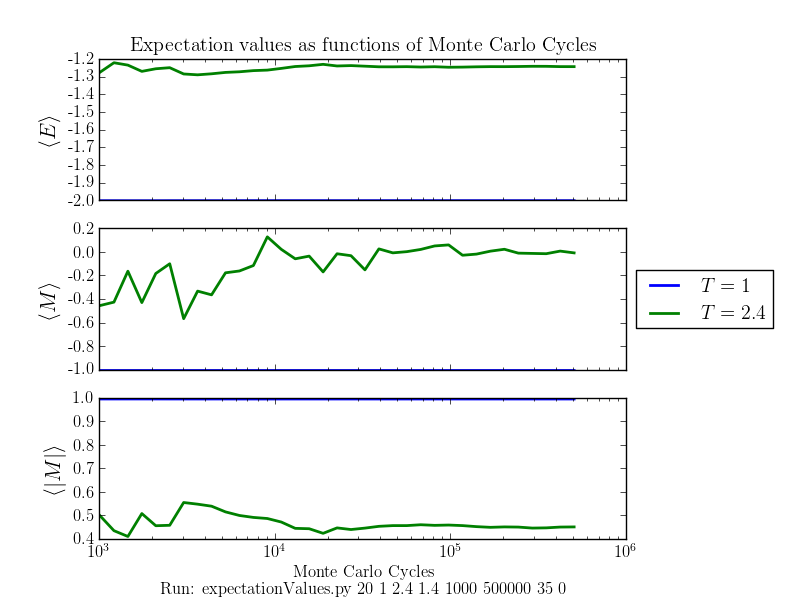
\includegraphics[scale=0.7]{../fig/E_M_Mabs.png}
  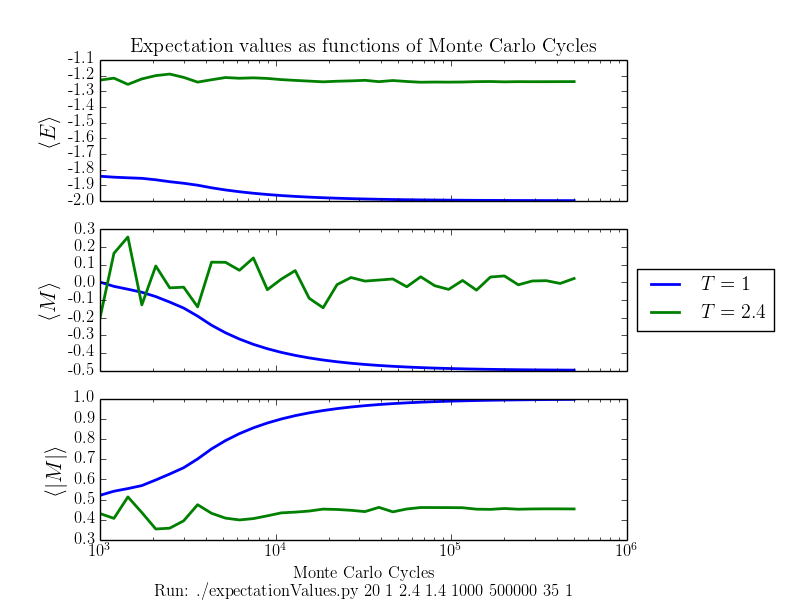
\includegraphics[scale=0.7]{../fig/E_M_Mabs_random.png}
  \caption{Plot av forventningsverdien til energi,
    magnetisering og absoluttverdien til magnetiseringa som funksjon av antall Monte Carlo-sykluser. 
    Øverst har vi det ordnede tilfellet der alle spins begynner med å peke ned. Det andre tilfellet er 
    med en tilfeldig startkonfigurasjon.}
\label{fig:forventningsverdi}
\end{figure*}


\begin{figure*}[ht]
  \centering
  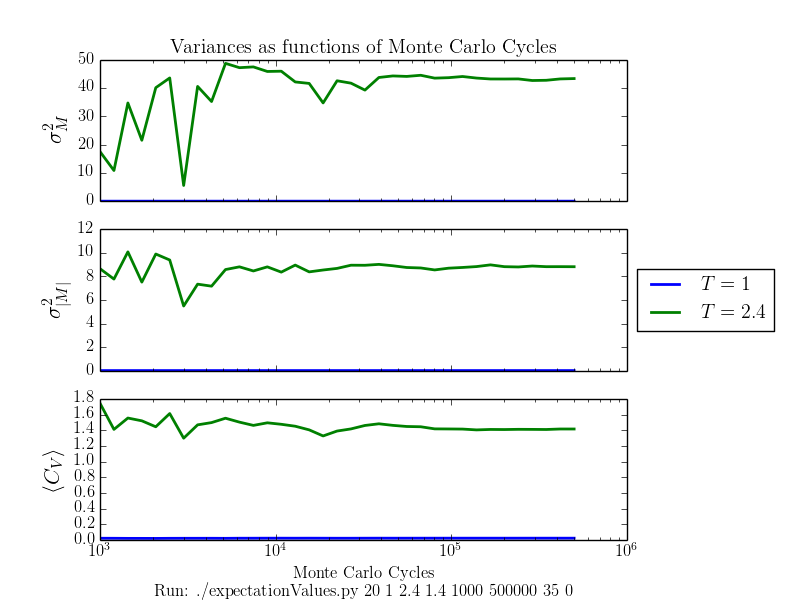
\includegraphics[scale=0.7]{../fig/variances.png}
  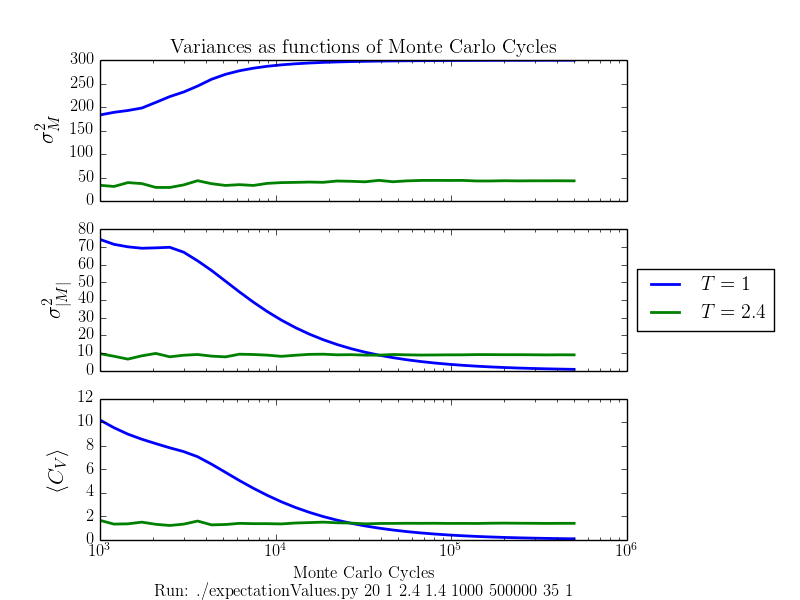
\includegraphics[scale=0.7]{../fig/variances_random.png}
  \caption{\label{fig:varianser} Plot av variansen til energien og magnetiseringa som
funksjon av antall Monte Carlo-sykluser. Variansen regner vi både med å bruke $\chi$ og $|\chi|$. Øverst
er det ordnete tilfellet, nederst det uordnede.}
\end{figure*}


\begin{figure*}[ht]
  \centering
  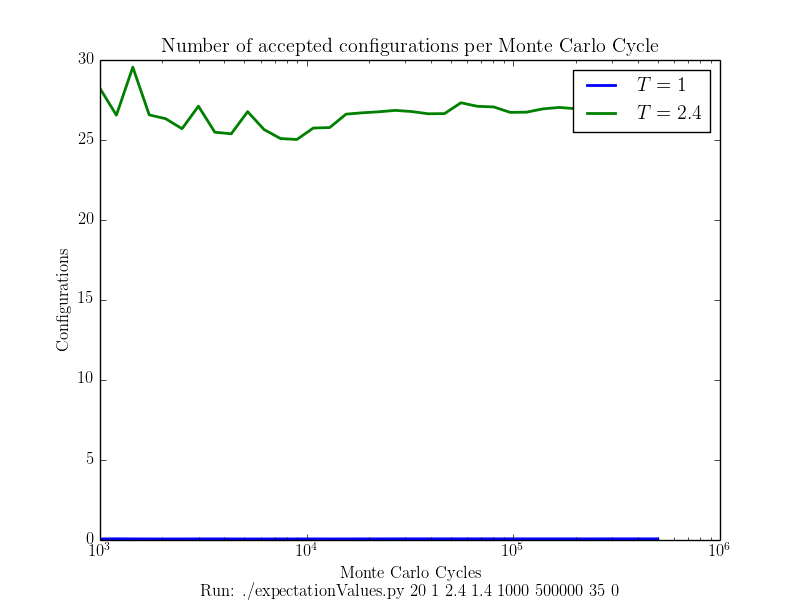
\includegraphics[scale=0.7]{../fig/configurations.png}
  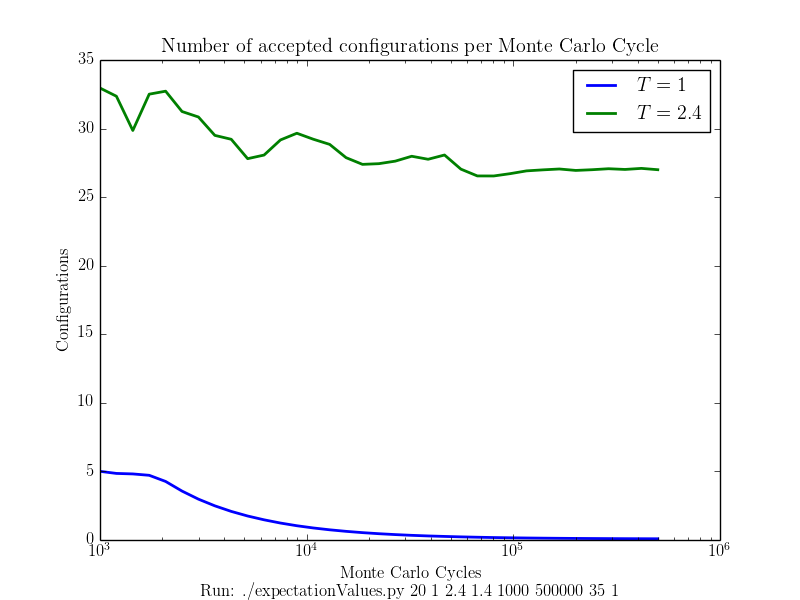
\includegraphics[scale=0.7]{../fig/configurations_random.png}
  \caption{\label{fig:configurations} Et plot av antall configurations
normalisert mot antall Monte Carlo-sykluser. Øverst er det ordnete tilfellet, nederst det uordnede.}
\end{figure*}

\subsubsection{Implementering av termalisering}
\label{subsec:implementering-av-termalisering}
Fra disse resultatene estimerer vi altså at vi burde starte
datasamlingen først etter ca. $3\e{4}$ sykluser. Et alternativ ville vært å bruke
dette som en gitt grense i programmet. Vi skal derimot forsøke en litt
mer robust metode:

Vi kan sammenlikne energien (og/eller andre størrelser vi beregner)
fra et tidligere punkt i simuleringen med en ny verdi si 1000 sykluser
etterpå. Dersom systemet ikke har nådd likevekt vil vi forvente å se
en betydelig endring av verdien, men dersom systemet har blitt
termalisert burde vi ikke se store svingninger. Derfor hvis verdiene ikke har endret
seg mer enn en gitt prosentandel på et visst antall sykluser så antar vi at
systemet er termalisert og vi kan begynne å samle data. Dette gjør vi
kun for den første temperaturen. For de resterende temperaturene lagrer
vi spinkonfigurasjonen fra det foregående temperatursteget og antar at hvis
modellen var termalisert for $T$, vil samme spinkonfigurasjon være tilnærmet
termalisert for $T+ \Delta T$.

Denne metoden er dessverre ikke idiotsikker. Først og fremst blir
det opp til oss å finne en passende grense for prosentandelen vi
tillater at endres. Dette er ikke så lett å gjøre generelt, ettersom
ulike temperaturer og startkonfigurasjoner vil bruke ulik tid på å nå
likevekt. Selv om vi finner en ideell verdi for denne kan det også hende
at vi bare ved en tilfeldighet ender med nye verdier som er veldig
like de vi hadde tidligere, selv om systemet ikke har nådd den mest
sannsynlige tilstanden. Dette er likevel svært usannsynlig, så vi
``krysser fingrene'' og håper på det beste.

Ved litt testing fant vi at en grense som så ut til å fungere for alle relevante
temperaturer var ca. $5\%$. Vi regner altså systemet som termalisert når
energien og magnetiseringen ikke endrer seg mer enn $5 \%$ på 1000 sykluser.\footnote{Programmet som inneholder termaliserings-implementasjonen heter \texttt{MPIisingImproved.cpp} og er
tilgjengelig på Github~\cite{github-repo}}

En enda mer robust metode ville f.eks. vært å bruke autokorrelasjonsfunksjonen,
men vi har valgt å ikke prioritere dette i denne omgang.

\subsubsection{Forbedringer med termalisering}
Som en test av denne implementasjonen har vi på nytt regnet ut
verdiene fra tabell \ref{tab:2x2-eksakt-num}. Denne gangen har vi satt
temperaturen til $T=2.3$, $L=2$ og brukt $10^6$ Monte
Carlo-sykluser. Det nye resultatet er vist i tabell \ref{tab:exact-numerical-improved}

\begin{table*}
\centering
\caption{Tabell over eksakte og numeriske resultater for $2\times
  2$-tilfellet for $T=2.3$. Vi har brukt $10^6$ Monte Carlo-sykluser og
  en startkonfigurasjon med alle spinn pekende ned, $\downarrow$. Merk at
alle tall er normalisert for antall spinn. Vi ser en forbedring
med programmet som tar hensyn til termalisering. Forbedringen er gitt
som hvor mange prosent større den relative feilen er for det
ikke-termaliserte resultatet.}
\label{tab:exact-numerical-improved}
\vspace{0.1cm}
\begin{tabular}{l|ccccc}
$T=2.3$ & $\mean{E}$ & $\mean{ \abs{\mathcal{M} } }$ & $C_V$ & $\chi$ & $\chi_\text{abs}$ \\
\hline
Eksakt          & -1.684566     & 0.89512301    & 0.40664873   & 1.5114861 & 0.11801616 \\
Standard        & -1.6852440    & 0.89540700    & 0.40572904   & 1.5119883 & 0.11764227 \\
Termalisert     & -1.6851001    & 0.89535794    & 0.40588694   & 1.5118878 & 0.11769110\\
Rel. feil std.  & $-4.02\e{-4}$ & $-3.17\e{-4}$ & $2.26\e{-3}$ & $3.32\e{-4}$ & $3.17\e{-3}$ \\
Rel. feil term. & $-3.17\e{-4}$ & $-2.62\e{-4}$ & $1.87\e{-3}$ &
                                                                 $-2.66\e{-4}$ & $2.75\e{-3}$\\
Forbedring  & 27\% & 21\% & 21\% & 25\% & 15\%
\end{tabular}
\end{table*}

Fra tabellen ser vi at vi har jevnt over en forbedring på ca. $20\%$ i
den relative feilen. Vi kunne trolig forbedret dette ytterligere ved å
finne en annen prosentgrense (fra seksjon
\ref{subsec:implementering-av-termalisering}), men vi begrenser oss
til å bruke en og samme verdi for alle temperaturer, verdier av
$L$ og/eller antall Monte Carlo-sykluser. 

\pagebreak
\section{Resultater}
Med programmet mer eller mindre ferdigkodet og -testet kan vi begynne
å se mer på egenskapene ved modellen.
\subsection{Sannsynlighetsfordeling}
Det er interessant å se hvilke
energier som forekommer for forskjellige temperaturer, og hvor mange ganger dette skjer.
I figur \ref{fig:probabilities} ser vi et histogram av tilstandene
for $L=20$ ved temperaturene $T=1$, $T=1.7$ og $T=2.4$. Vi ser at ved lav temperatur
skjer det relativt lite i systemet, og vi har få tilstandsendringer. 
Dette er tilsvarende
det vi så i figur \ref{fig:configurations}. Ved høyere temperatur ser vi derimot
at vi har mange tilgjengelige tilstander for systemet, og 
sannsynlighetsfordelingen ser veldig ut som en Boltzmann-fordeling.

Programmet som lager histogrammet, \texttt{probabilities.py}, skriver
også ut varmekapasiteten ved hjelp av variansen til datasettet. Vi kan
sammenlikne disse verdiene med forventningsverdien som blir
beregnet. Tabell \ref{tab:var-vs-Cv} viser dette. Vi ser (slik vi
burde) at disse to beregningene gir lignende svar. 

\begin{table*}
\centering
\caption{Tabellen viser varmekapasiteten beregnet fra variansen i
  histogrammet i figur \ref{fig:probabilities} og verdien som beregnes
av \texttt{MPIisingimproved.cpp}.}
\label{tab:var-vs-Cv}
\vspace{0.1cm}
\begin{tabular}{c|cc}
hei &\texttt{MPIisingimproved.cpp} & Varians i histogram\\
\hline
$T=1.0$ & 0.01033735  & 0.023351\\
$T=1.7$ & 0.34147839  & 0.348439 \\
$T=2.4$ & 1.4264178 & 1.40566
\end{tabular}
\end{table*}

\begin{figure*}[ht]
  \centering
  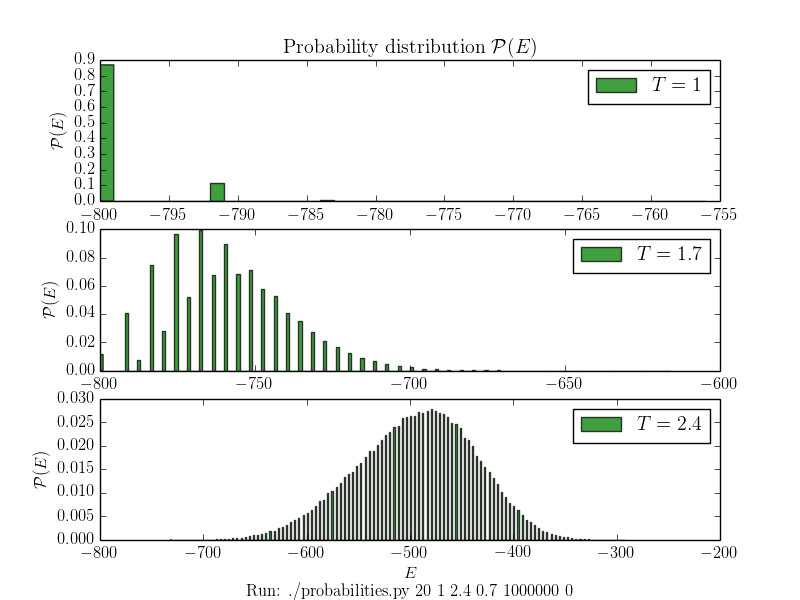
\includegraphics[scale=0.7]{../fig/prob_E.png}
  \caption{Et histogram av tilstandene for $L=20$ ved tre
forskjellige temperaturer. Vi ser at ved lav temperatur
skjer det relativt lite i systemet, og vi har få tilstands-hopp. Ved høyere temperatur ser vi derimot at vi har mange tilgjengelige tilstander for systemet, og 
sannsynlighetsfordelingen ser veldig ut som en Boltzmann-fordeling.}
\label{fig:probabilities}
\end{figure*}



\subsection{Beregning av kritisk temperatur}
En sentral størrelse for dette systemet er den kritiske temperaturen
$T_C$. Rundt denne temperaturen kan vi beskrive mange fysiske
størrelser ved hjelp av potenslover. Eksempelvis er
forventningsverdien til magnetiseringen gitt som 
\begin{align}
  \mean{\mathcal{M}(T)} \sim (T - T_C)^{\beta},
\end{align}
der $\beta=1/8$ er en såkalt kritisk eksponent. Vi har en lignende
relasjon for varmekapasiteten,
\begin{align}
  C_V(T) \sim |T-T_C|^{\alpha},
\end{align}
og susceptibiliteten,
\begin{align}
  \chi(T) \sim |T_C - T|^{\gamma}.
\end{align}
med $\alpha=0$ og $\gamma=7/4$.

En annen viktig størrelse er korrelasjonslengden $\xi$, som er i
størrelsesorden lik avstanden mellom spinnene for $T\gg T_C$. Spinnene
vil bli stadig mer korrelert når temperaturen nærmer seg $T_C$, som
svarer til at $\xi$ vokser når $T\rightarrow T_C$. Den divergente
oppførselen til $\xi$ rundt $T_C$ er igjen gitt ved en potenslov:
\begin{align}
  \xi(T) \sim |T_C - T|^\nu.\label{eq:corr-length-critical}
\end{align}
En andreordens faseovergang karakteriseres av en korrelasjonslengde
som spenner hele systemet. I en slik overgang er derfor
korrelasjonslengden proporsjonal med størrelsen på
spinn-rutenettet. Vi vil alltid være begrenset til å se på et endelig
rutenett, men ved såkalt ``finite size scaling relation'' er det mulig
å knytte oppførselen til endelig-dimensjonale rutenett til den
termodynamiske grensen der $L\rightarrow\infty$. For den kritiske
temperaturen er denne skaleringen gitt som 
\begin{align}
  T_C(L) - T_C(L=\infty) = aL^{-1/\nu}\label{eq:Tc-scaling},
\end{align} 
der $a$ er en konstant og $\nu$ definert i likning \eqref{eq:corr-length-critical}.  Vi kan sette
$\nu=1$~\cite{oppgavetekst-prosjekt-4}. 

\vspace{\baselineskip}

Med utgangspunkt i likning \eqref{eq:Tc-scaling} kan vi beregne den
kritiske temperaturen for noen endelige verdier av $L$ og bruke dem
til å finne verdien når $L\rightarrow\infty$. Vi ser at vi har en
ukjent $a$, så vi trenger å beregne for to verdier av $L$ slik at vi
får to likninger med to ukjente. Altså,

\begin{align}
  &T_C(L_1) - T_C(L=\infty) = aL_1^{-1/\nu}\\
  &T_C(L_2) - T_C(L=\infty) = aL_2^{-1/\nu}\\
\Rightarrow &a = \frac{ T_C(L_1) - T_C(L_2)} {L_1^{-1/\nu} -
  L_2^{-1/\nu}}\\
\begin{split}
\Rightarrow &T_C(L=\infty) = \\ &T_C(L_1) - \frac{ T_C(L_1) - T_C(L_2)} {L_1^{-1/\nu} -
  L_2^{-1/\nu}}L_1^{-1/\nu}\label{eq:Tc-inf-scale-expression}.
\end{split}
\end{align}
Det eneste som gjenstår nå er å bestemme $T_C(L)$ ut fra
beregningene. Vi har laget et program som genererer plott for
forventningsverdiene $\mean{E}$, $\mean{\abs{\mathcal{M}}}$, $C_V$ og
$\chi_\text{abs}$ som funksjoner av temperatur. Programmet heter
\texttt{critical.py} og er tilgjengelig på
Github~\cite{github-repo}. Resultatene er vist i figur \ref{fig:critical-plot} (merk at
parameterene brukt til å lage plottet er vist på undersiden av
figuren). 

\begin{figure*}[ht]
  \centering
  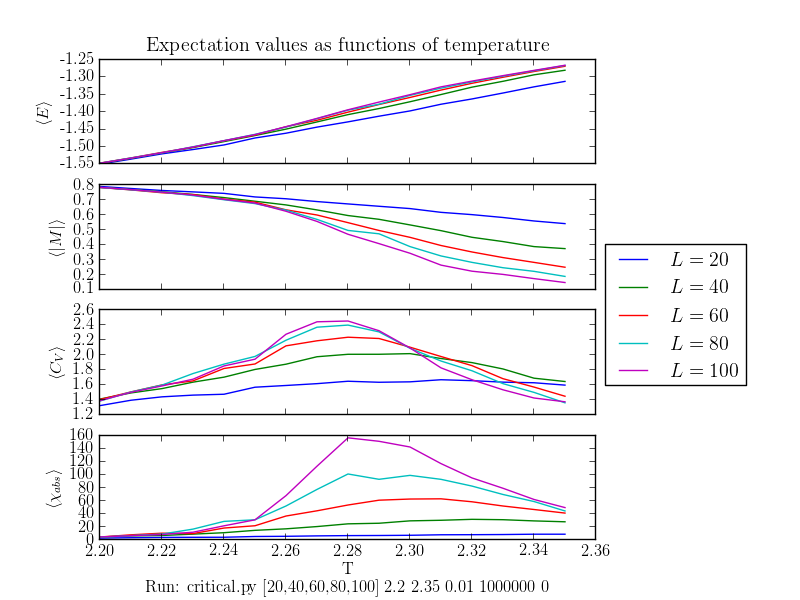
\includegraphics[scale=0.7]{../fig/critical.png}
  \caption{\label{fig:critical-plot} Forventningsverdier som funksjon
    av temperatur. Vi observerer en faseovergang rundt en kritisk
    temperatur, og merker oss at toppene til $C_V(T)$ og
    $\chi_\text{abs}(T)$ blir stadig høyere for større verdier av
    $L$. Selv om det ikke er veldig tydelig ser vi også antydning til
    vendepunkter ved kritisk temperatur for $\mean{E}$ og
    $\mean{|\mathcal{M}|}$. Vi kan også merke oss at oppløsningen i
    $T$ burde vært større dersom vi hadde ønsket et bedre estimat for
    $T_C(L=\infty)$.}
\end{figure*}

Figuren minner oss om at $C_V \propto \pd{E}{T}$ og $\chi_\text{abs}
\propto \pd{\abs{M}}{T}$ ettersom vi har maksima for disse størrelsene
der vendepunktene er. Vi vet videre at $\mathcal{M}$ skal gå i
en sirkel fra $\mathcal{M}(T=0)=1$ til $\mathcal{M}(T\geq T_C)=0$ i
grensen $L\rightarrow\infty$~\cite{ising-model-texas-uni}. Desto
større $L$, desto fortere vil verdien synke mot null ved den kritiske
temperaturen. Vi ser antydning til denne tendensen, men er langt fra
en sirkelform. Dette har selvsagt med å gjøre at er begrenset til et
relativt lite rutenett. 

Vi observerer at $\chi_\text{abs}$ har den tydeligeste toppen, og
bruker derfor denne størrelsen når vi skal bestemme verdien til
$T_C(L)$. Dette er da enkelt temperaturen der $\chi_\text{abs}$ er
maksimal. Gjør vi dette for to verdier av $L$ (gjerne de to største vi
har kjørt for siden disse har tydeligst maksima) kan vi bruke likning
\eqref{eq:Tc-inf-scale-expression} og finne et estimat for den
kritiske temperaturen i den termodynamiske grensen. Programmet
\texttt{critical.py} automatiserer denne beregningen og gir oss
resultatet. Med parametere som vist i figur \ref{fig:critical-plot}
får vi et estimat
\begin{align}
  T_C(L=\infty)_\text{approx} = 2.28
\end{align}

Vi kan sammenlikne resultatet med Lars Onsagers analytiske resultat~\cite{oppgavetekst-prosjekt-4},
\begin{align}
\begin{split}
  kT_C(L=\infty)/J &= \frac{ 2 }{ \ln \left( 1+\sqrt{2} \right) }\\
  &\approx 2.269
\end{split}
\end{align}

Vi ser at vår tilnærming ikke er helt på mål, men likevel ikke veldig
langt unna heller. Vi må bemerke at resultatene våre hadde hatt godt
av en større oppløsning i $T$, og det kan godt hende at vi hadde
oppnådd et mye mer presist resultat dersom vi hadde tid til å kjøre en
større simulering. Vi hadde dessverre en programmeringsfeil som ikke
ble oppdaget før samme dag som innleveringsfristen. Dette gjorde at
alle tidligere datasett måtte regnes ut på nytt, og vi hadde dermed
ikke mulighet til å la en maskin stå over natten (slik vi hadde gjort i
forkant av oppdagelsen av feilen). 

\section{Konklusjon}


\clearpage
\onecolumn
\printbibliography
\end{document}
%%% Local Variables:
%%% mode: latex
%%% TeX-master: t
%%% End:
